\documentclass[10pt,a4paper]{article}\usepackage[]{graphicx}\usepackage[]{color}
%% maxwidth is the original width if it is less than linewidth
%% otherwise use linewidth (to make sure the graphics do not exceed the margin)
\makeatletter
\def\maxwidth{ %
  \ifdim\Gin@nat@width>\linewidth
    \linewidth
  \else
    \Gin@nat@width
  \fi
}
\makeatother

\definecolor{fgcolor}{rgb}{0.345, 0.345, 0.345}
\newcommand{\hlnum}[1]{\textcolor[rgb]{0.686,0.059,0.569}{#1}}%
\newcommand{\hlstr}[1]{\textcolor[rgb]{0.192,0.494,0.8}{#1}}%
\newcommand{\hlcom}[1]{\textcolor[rgb]{0.678,0.584,0.686}{\textit{#1}}}%
\newcommand{\hlopt}[1]{\textcolor[rgb]{0,0,0}{#1}}%
\newcommand{\hlstd}[1]{\textcolor[rgb]{0.345,0.345,0.345}{#1}}%
\newcommand{\hlkwa}[1]{\textcolor[rgb]{0.161,0.373,0.58}{\textbf{#1}}}%
\newcommand{\hlkwb}[1]{\textcolor[rgb]{0.69,0.353,0.396}{#1}}%
\newcommand{\hlkwc}[1]{\textcolor[rgb]{0.333,0.667,0.333}{#1}}%
\newcommand{\hlkwd}[1]{\textcolor[rgb]{0.737,0.353,0.396}{\textbf{#1}}}%

\usepackage{framed}
\makeatletter
\newenvironment{kframe}{%
 \def\at@end@of@kframe{}%
 \ifinner\ifhmode%
  \def\at@end@of@kframe{\end{minipage}}%
  \begin{minipage}{\columnwidth}%
 \fi\fi%
 \def\FrameCommand##1{\hskip\@totalleftmargin \hskip-\fboxsep
 \colorbox{shadecolor}{##1}\hskip-\fboxsep
     % There is no \\@totalrightmargin, so:
     \hskip-\linewidth \hskip-\@totalleftmargin \hskip\columnwidth}%
 \MakeFramed {\advance\hsize-\width
   \@totalleftmargin\z@ \linewidth\hsize
   \@setminipage}}%
 {\par\unskip\endMakeFramed%
 \at@end@of@kframe}
\makeatother

\definecolor{shadecolor}{rgb}{.97, .97, .97}
\definecolor{messagecolor}{rgb}{0, 0, 0}
\definecolor{warningcolor}{rgb}{1, 0, 1}
\definecolor{errorcolor}{rgb}{1, 0, 0}
\newenvironment{knitrout}{}{} % an empty environment to be redefined in TeX

\usepackage{alltt}

\usepackage[T1]{fontenc}
\usepackage[polish]{babel}
\usepackage[cp1250]{inputenc}
\usepackage{amsmath}
\usepackage{amsfonts}
\usepackage{graphicx}
\usepackage{setspace}
\usepackage{savesym}
\savesymbol{arc}
\usepackage{color}
\usepackage{xcolor}
\usepackage{pict2e}
\usepackage{epstopdf}
\usepackage{geometry}

\newgeometry{tmargin=1cm, bmargin=1cm, lmargin=1cm, rmargin=1cm}
\pagestyle{empty}
\linespread{1.2}
\IfFileExists{upquote.sty}{\usepackage{upquote}}{}

\begin{document}

\subsection*{\textbf{Zadanie 2.1}}

\begin{knitrout}
\definecolor{shadecolor}{rgb}{0.969, 0.969, 0.969}\color{fgcolor}\begin{kframe}
\begin{alltt}
\hlcom{# 2.1}

\hlkwd{library}\hlstd{(}\hlstr{"klaR"}\hlstd{)}
\hlkwd{library}\hlstd{(}\hlstr{"MASS"}\hlstd{)}

\hlstd{w} \hlkwb{<-} \hlkwd{read.table}\hlstd{(}\hlstr{"http://www.ipipan.eu/~teisseyrep/TEACHING/DM/DANE/wine.data"}\hlstd{,}
    \hlkwc{sep} \hlstd{=} \hlstr{","}\hlstd{)}
\hlkwd{head}\hlstd{(w,} \hlnum{2}\hlstd{)}
\end{alltt}
\begin{verbatim}
##   V1    V2   V3   V4   V5  V6   V7   V8   V9  V10  V11  V12  V13  V14
## 1  1 14.23 1.71 2.43 15.6 127 2.80 3.06 0.28 2.29 5.64 1.04 3.92 1065
## 2  1 13.20 1.78 2.14 11.2 100 2.65 2.76 0.26 1.28 4.38 1.05 3.40 1050
\end{verbatim}
\begin{alltt}
\hlcom{# a)}

\hlstd{m1} \hlkwb{<-} \hlkwd{lda}\hlstd{(V1} \hlopt{~} \hlstd{V2} \hlopt{+} \hlstd{V8,} \hlkwc{data} \hlstd{= w)}
\hlstd{z1} \hlkwb{<-} \hlkwd{predict}\hlstd{(m1,} \hlkwc{newdata} \hlstd{= w)}\hlopt{$}\hlstd{posterior}
\hlkwd{head}\hlstd{(z1,} \hlnum{2}\hlstd{)}  \hlcom{# pstwo aposteriori}
\end{alltt}
\begin{verbatim}
##        1         2         3
## 1 0.9996 0.0003965 2.206e-05
## 2 0.8124 0.1866492 9.655e-04
\end{verbatim}
\begin{alltt}
\hlcom{# b)}

\hlstd{klasy} \hlkwb{<-} \hlkwd{predict}\hlstd{(m1,} \hlkwc{newdata} \hlstd{= w)}\hlopt{$}\hlstd{class}
\hlstd{t} \hlkwb{<-} \hlkwd{table}\hlstd{(w}\hlopt{$}\hlstd{V1, klasy)}
\hlstd{t}
\end{alltt}
\begin{verbatim}
##    klasy
##      1  2  3
##   1 56  3  0
##   2  4 60  7
##   3  0  0 48
\end{verbatim}
\begin{alltt}
\hlnum{100} \hlopt{*} \hlkwd{sum}\hlstd{(}\hlkwd{diag}\hlstd{(t))}\hlopt{/}\hlkwd{nrow}\hlstd{(w)}  \hlcom{# procent poprawnych klasyfikacji}
\end{alltt}
\begin{verbatim}
## [1] 92.13
\end{verbatim}
\begin{alltt}
\hlcom{# c)}

\hlstd{n1} \hlkwb{<-} \hlkwd{length}\hlstd{(}\hlkwd{which}\hlstd{(w}\hlopt{$}\hlstd{V1} \hlopt{==} \hlnum{1}\hlstd{))}
\hlstd{n2} \hlkwb{<-} \hlkwd{length}\hlstd{(}\hlkwd{which}\hlstd{(w}\hlopt{$}\hlstd{V1} \hlopt{==} \hlnum{2}\hlstd{))}
\hlstd{n3} \hlkwb{<-} \hlkwd{length}\hlstd{(}\hlkwd{which}\hlstd{(w}\hlopt{$}\hlstd{V1} \hlopt{==} \hlnum{3}\hlstd{))}

\hlkwd{plot}\hlstd{(w}\hlopt{$}\hlstd{V2, w}\hlopt{$}\hlstd{V8,} \hlkwc{xlab} \hlstd{=} \hlstr{"alkohol"}\hlstd{,} \hlkwc{ylab} \hlstd{=} \hlstr{"flawonidy"}\hlstd{,} \hlkwc{pch} \hlstd{=} \hlkwd{c}\hlstd{(}\hlkwd{rep}\hlstd{(}\hlstr{"1"}\hlstd{, n1),}
    \hlkwd{rep}\hlstd{(}\hlstr{"2"}\hlstd{, n2),} \hlkwd{rep}\hlstd{(}\hlstr{"3"}\hlstd{, n3)),} \hlkwc{col} \hlstd{=} \hlkwd{c}\hlstd{(}\hlkwd{rep}\hlstd{(}\hlstr{"red"}\hlstd{, n1),} \hlkwd{rep}\hlstd{(}\hlstr{"blue"}\hlstd{, n2),} \hlkwd{rep}\hlstd{(}\hlstr{"green"}\hlstd{,}
    \hlstd{n3)))}

\hlstd{x} \hlkwb{<-} \hlkwd{seq}\hlstd{(}\hlnum{10.5}\hlstd{,} \hlnum{15.5}\hlstd{,} \hlkwc{length.out} \hlstd{=} \hlnum{200}\hlstd{)}
\hlstd{y} \hlkwb{<-} \hlkwd{seq}\hlstd{(}\hlnum{0}\hlstd{,} \hlnum{5.5}\hlstd{,} \hlkwc{length.out} \hlstd{=} \hlnum{200}\hlstd{)}
\hlstd{siatka} \hlkwb{<-} \hlkwd{expand.grid}\hlstd{(}\hlkwc{V2} \hlstd{= x,} \hlkwc{V8} \hlstd{= y)}
\hlstd{pred} \hlkwb{<-} \hlkwd{predict}\hlstd{(m1,} \hlkwc{newdata} \hlstd{= siatka)}\hlopt{$}\hlstd{posterior}

\hlstd{z1} \hlkwb{<-} \hlstd{pred[,} \hlnum{1}\hlstd{]} \hlopt{-} \hlkwd{pmax}\hlstd{(pred[,} \hlnum{2}\hlstd{], pred[,} \hlnum{3}\hlstd{])}
\hlstd{z2} \hlkwb{<-} \hlstd{pred[,} \hlnum{2}\hlstd{]} \hlopt{-} \hlkwd{pmax}\hlstd{(pred[,} \hlnum{1}\hlstd{], pred[,} \hlnum{3}\hlstd{])}
\hlstd{z3} \hlkwb{<-} \hlstd{pred[,} \hlnum{3}\hlstd{]} \hlopt{-} \hlkwd{pmax}\hlstd{(pred[,} \hlnum{2}\hlstd{], pred[,} \hlnum{1}\hlstd{])}

\hlkwd{contour}\hlstd{(x, y,} \hlkwd{matrix}\hlstd{(z1,} \hlnum{200}\hlstd{),} \hlkwc{level} \hlstd{=} \hlnum{0}\hlstd{,} \hlkwc{add} \hlstd{= T)}
\hlkwd{contour}\hlstd{(x, y,} \hlkwd{matrix}\hlstd{(z2,} \hlnum{200}\hlstd{),} \hlkwc{level} \hlstd{=} \hlnum{0}\hlstd{,} \hlkwc{add} \hlstd{= T)}
\hlkwd{contour}\hlstd{(x, y,} \hlkwd{matrix}\hlstd{(z3,} \hlnum{200}\hlstd{),} \hlkwc{level} \hlstd{=} \hlnum{0}\hlstd{,} \hlkwc{add} \hlstd{= T)}
\end{alltt}
\end{kframe}

{\centering \includegraphics[width=\maxwidth]{figure/unnamed-chunk-11} 

}


\begin{kframe}\begin{alltt}
\hlkwd{partimat}\hlstd{(}\hlkwd{as.factor}\hlstd{(V1)} \hlopt{~} \hlstd{V8} \hlopt{+} \hlstd{V2,} \hlkwc{data} \hlstd{= w)}  \hlcom{# albo inaczej}
\end{alltt}
\end{kframe}

{\centering 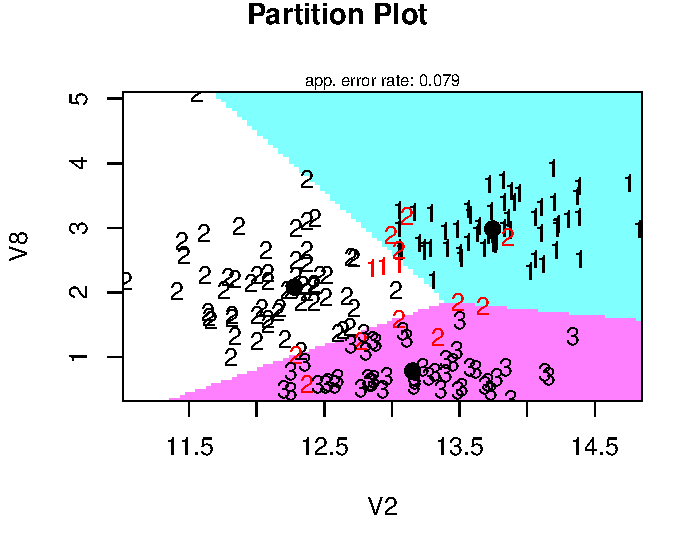
\includegraphics[width=\maxwidth]{figure/unnamed-chunk-12} 

}


\begin{kframe}\begin{alltt}
\hlcom{# d)}

\hlstd{m2} \hlkwb{<-} \hlkwd{qda}\hlstd{(V1} \hlopt{~} \hlstd{V2} \hlopt{+} \hlstd{V8,} \hlkwc{data} \hlstd{= w)}
\hlstd{z1} \hlkwb{<-} \hlkwd{predict}\hlstd{(m2,} \hlkwc{newdata} \hlstd{= w)}\hlopt{$}\hlstd{posterior}
\hlkwd{head}\hlstd{(z1,} \hlnum{2}\hlstd{)}
\end{alltt}
\begin{verbatim}
##        1         2         3
## 1 0.9996 0.0004125 4.547e-14
## 2 0.8735 0.1265091 1.904e-10
\end{verbatim}
\begin{alltt}
\hlstd{klasy} \hlkwb{<-} \hlkwd{predict}\hlstd{(m2,} \hlkwc{newdata} \hlstd{= w)}\hlopt{$}\hlstd{class}
\hlstd{t} \hlkwb{<-} \hlkwd{table}\hlstd{(w}\hlopt{$}\hlstd{V1, klasy)}
\hlstd{t}
\end{alltt}
\begin{verbatim}
##    klasy
##      1  2  3
##   1 57  2  0
##   2  4 65  2
##   3  0  3 45
\end{verbatim}
\begin{alltt}
\hlnum{100} \hlopt{*} \hlkwd{sum}\hlstd{(}\hlkwd{diag}\hlstd{(t))}\hlopt{/}\hlkwd{nrow}\hlstd{(w)}  \hlcom{# wiekszy niz w lda}
\end{alltt}
\begin{verbatim}
## [1] 93.82
\end{verbatim}
\begin{alltt}
\hlstd{n1} \hlkwb{<-} \hlkwd{length}\hlstd{(}\hlkwd{which}\hlstd{(w}\hlopt{$}\hlstd{V1} \hlopt{==} \hlnum{1}\hlstd{))}
\hlstd{n2} \hlkwb{<-} \hlkwd{length}\hlstd{(}\hlkwd{which}\hlstd{(w}\hlopt{$}\hlstd{V1} \hlopt{==} \hlnum{2}\hlstd{))}
\hlstd{n3} \hlkwb{<-} \hlkwd{length}\hlstd{(}\hlkwd{which}\hlstd{(w}\hlopt{$}\hlstd{V1} \hlopt{==} \hlnum{3}\hlstd{))}

\hlkwd{plot}\hlstd{(w}\hlopt{$}\hlstd{V2, w}\hlopt{$}\hlstd{V8,} \hlkwc{xlab} \hlstd{=} \hlstr{"alkohol"}\hlstd{,} \hlkwc{ylab} \hlstd{=} \hlstr{"flawonidy"}\hlstd{,} \hlkwc{pch} \hlstd{=} \hlkwd{c}\hlstd{(}\hlkwd{rep}\hlstd{(}\hlstr{"1"}\hlstd{, n1),}
    \hlkwd{rep}\hlstd{(}\hlstr{"2"}\hlstd{, n2),} \hlkwd{rep}\hlstd{(}\hlstr{"3"}\hlstd{, n3)),} \hlkwc{col} \hlstd{=} \hlkwd{c}\hlstd{(}\hlkwd{rep}\hlstd{(}\hlstr{"red"}\hlstd{, n1),} \hlkwd{rep}\hlstd{(}\hlstr{"blue"}\hlstd{, n2),} \hlkwd{rep}\hlstd{(}\hlstr{"green"}\hlstd{,}
    \hlstd{n3)))}

\hlstd{x} \hlkwb{<-} \hlkwd{seq}\hlstd{(}\hlnum{10.5}\hlstd{,} \hlnum{15.5}\hlstd{,} \hlkwc{length.out} \hlstd{=} \hlnum{200}\hlstd{)}
\hlstd{y} \hlkwb{<-} \hlkwd{seq}\hlstd{(}\hlnum{0}\hlstd{,} \hlnum{5.5}\hlstd{,} \hlkwc{length.out} \hlstd{=} \hlnum{200}\hlstd{)}
\hlstd{siatka} \hlkwb{<-} \hlkwd{expand.grid}\hlstd{(}\hlkwc{V2} \hlstd{= x,} \hlkwc{V8} \hlstd{= y)}
\hlstd{pred} \hlkwb{<-} \hlkwd{predict}\hlstd{(m2,} \hlkwc{newdata} \hlstd{= siatka)}\hlopt{$}\hlstd{posterior}

\hlstd{z1} \hlkwb{<-} \hlstd{pred[,} \hlnum{1}\hlstd{]} \hlopt{-} \hlkwd{pmax}\hlstd{(pred[,} \hlnum{2}\hlstd{], pred[,} \hlnum{3}\hlstd{])}
\hlstd{z2} \hlkwb{<-} \hlstd{pred[,} \hlnum{2}\hlstd{]} \hlopt{-} \hlkwd{pmax}\hlstd{(pred[,} \hlnum{1}\hlstd{], pred[,} \hlnum{3}\hlstd{])}
\hlstd{z3} \hlkwb{<-} \hlstd{pred[,} \hlnum{3}\hlstd{]} \hlopt{-} \hlkwd{pmax}\hlstd{(pred[,} \hlnum{2}\hlstd{], pred[,} \hlnum{1}\hlstd{])}

\hlkwd{contour}\hlstd{(x, y,} \hlkwd{matrix}\hlstd{(z1,} \hlnum{200}\hlstd{),} \hlkwc{level} \hlstd{=} \hlnum{0}\hlstd{,} \hlkwc{add} \hlstd{= T)}
\hlkwd{contour}\hlstd{(x, y,} \hlkwd{matrix}\hlstd{(z2,} \hlnum{200}\hlstd{),} \hlkwc{level} \hlstd{=} \hlnum{0}\hlstd{,} \hlkwc{add} \hlstd{= T)}
\hlkwd{contour}\hlstd{(x, y,} \hlkwd{matrix}\hlstd{(z3,} \hlnum{200}\hlstd{),} \hlkwc{level} \hlstd{=} \hlnum{0}\hlstd{,} \hlkwc{add} \hlstd{= T)}
\end{alltt}
\end{kframe}

{\centering \includegraphics[width=\maxwidth]{figure/unnamed-chunk-13} 

}



\end{knitrout}


\subsection*{\textbf{Zadanie 2.2}}

\begin{knitrout}
\definecolor{shadecolor}{rgb}{0.969, 0.969, 0.969}\color{fgcolor}\begin{kframe}
\begin{alltt}
\hlcom{# 2.2}

\hlstd{m} \hlkwb{<-} \hlkwd{read.table}\hlstd{(}\hlstr{"http://www.ipipan.eu/~teisseyrep/TEACHING/DM/DANE/kredit.asc"}\hlstd{,}
    \hlkwc{header} \hlstd{=} \hlnum{TRUE}\hlstd{)}
\hlkwd{head}\hlstd{(m,} \hlnum{2}\hlstd{)}
\end{alltt}
\begin{verbatim}
##   kredit laufkont laufzeit moral verw hoehe sparkont beszeit rate famges
## 1      1        1       18     4    2  1049        1       2    4      2
## 2      1        1        9     4    0  2799        1       3    2      3
##   buerge wohnzeit verm alter weitkred wohn bishkred beruf pers telef
## 1      1        4    2    21        3    1        1     3    1     1
## 2      1        2    1    36        3    1        2     3    2     1
##   gastarb
## 1       1
## 2       1
\end{verbatim}
\begin{alltt}
\hlcom{# a)}

\hlstd{m_lda} \hlkwb{<-} \hlkwd{lda}\hlstd{(kredit} \hlopt{~} \hlstd{.,} \hlkwc{data} \hlstd{= m)}
\hlstd{m_qda} \hlkwb{<-} \hlkwd{qda}\hlstd{(kredit} \hlopt{~} \hlstd{.,} \hlkwc{data} \hlstd{= m)}

\hlstd{t_lda} \hlkwb{<-} \hlkwd{table}\hlstd{(m}\hlopt{$}\hlstd{kredit,} \hlkwd{predict}\hlstd{(m_lda,} \hlkwc{newdata} \hlstd{= m)}\hlopt{$}\hlstd{class)}
\hlstd{t_lda}
\end{alltt}
\begin{verbatim}
##    
##       0   1
##   0 149 151
##   1  79 621
\end{verbatim}
\begin{alltt}
\hlnum{100} \hlopt{*} \hlkwd{sum}\hlstd{(}\hlkwd{diag}\hlstd{(t_lda))}\hlopt{/}\hlkwd{nrow}\hlstd{(m)}
\end{alltt}
\begin{verbatim}
## [1] 77
\end{verbatim}
\begin{alltt}
\hlstd{t_qda} \hlkwb{<-} \hlkwd{table}\hlstd{(m}\hlopt{$}\hlstd{kredit,} \hlkwd{predict}\hlstd{(m_qda,} \hlkwc{newdata} \hlstd{= m)}\hlopt{$}\hlstd{class)}
\hlstd{t_qda}
\end{alltt}
\begin{verbatim}
##    
##       0   1
##   0 200 100
##   1 121 579
\end{verbatim}
\begin{alltt}
\hlnum{100} \hlopt{*} \hlkwd{sum}\hlstd{(}\hlkwd{diag}\hlstd{(t_qda))}\hlopt{/}\hlkwd{nrow}\hlstd{(m)}
\end{alltt}
\begin{verbatim}
## [1] 77.9
\end{verbatim}
\end{kframe}
\end{knitrout}


\begin{knitrout}
\definecolor{shadecolor}{rgb}{0.969, 0.969, 0.969}\color{fgcolor}\begin{kframe}
\begin{alltt}
\hlcom{# b)}

\hlstd{s_lda} \hlkwb{<-} \hlkwd{stepclass}\hlstd{(m[,} \hlnum{2}\hlopt{:}\hlkwd{ncol}\hlstd{(m)], m[,} \hlnum{1}\hlstd{],} \hlkwc{method} \hlstd{=} \hlstr{"lda"}\hlstd{,} \hlkwc{direction} \hlstd{=} \hlstr{"backward"}\hlstd{)}
\end{alltt}
\end{kframe}
\end{knitrout}


\begin{knitrout}
\definecolor{shadecolor}{rgb}{0.969, 0.969, 0.969}\color{fgcolor}\begin{kframe}
\begin{alltt}
\hlstd{s_lda}\hlopt{$}\hlstd{formula}
\end{alltt}
\begin{verbatim}
## m[, 1] ~ laufkont + laufzeit + moral + verw + sparkont + beszeit + 
##     rate + famges + buerge + wohnzeit + verm + alter + weitkred + 
##     wohn + bishkred + telef + gastarb
## <environment: 0x000000000da72d30>
\end{verbatim}
\begin{alltt}
\hlstd{m_lda2} \hlkwb{<-} \hlkwd{lda}\hlstd{(s_lda}\hlopt{$}\hlstd{formula,} \hlkwc{data} \hlstd{= m)}
\hlstd{t_lda2} \hlkwb{<-} \hlkwd{table}\hlstd{(m}\hlopt{$}\hlstd{kredit,} \hlkwd{predict}\hlstd{(m_lda2,} \hlkwc{newdata} \hlstd{= m)}\hlopt{$}\hlstd{class)}
\hlstd{t_lda2}
\end{alltt}
\begin{verbatim}
##    
##       0   1
##   0 150 150
##   1  74 626
\end{verbatim}
\begin{alltt}
\hlnum{100} \hlopt{*} \hlkwd{sum}\hlstd{(}\hlkwd{diag}\hlstd{(t_lda2))}\hlopt{/}\hlkwd{nrow}\hlstd{(m)}
\end{alltt}
\begin{verbatim}
## [1] 77.6
\end{verbatim}
\end{kframe}
\end{knitrout}


\begin{knitrout}
\definecolor{shadecolor}{rgb}{0.969, 0.969, 0.969}\color{fgcolor}\begin{kframe}
\begin{alltt}
\hlstd{s_qda} \hlkwb{<-} \hlkwd{stepclass}\hlstd{(m[,} \hlnum{2}\hlopt{:}\hlkwd{ncol}\hlstd{(m)], m[,} \hlnum{1}\hlstd{],} \hlkwc{method} \hlstd{=} \hlstr{"qda"}\hlstd{,} \hlkwc{direction} \hlstd{=} \hlstr{"backward"}\hlstd{)}
\end{alltt}
\end{kframe}
\end{knitrout}


\begin{knitrout}
\definecolor{shadecolor}{rgb}{0.969, 0.969, 0.969}\color{fgcolor}\begin{kframe}
\begin{alltt}
\hlstd{s_qda}\hlopt{$}\hlstd{formula}
\end{alltt}
\begin{verbatim}
## m[, 1] ~ laufkont + laufzeit + moral + verw + hoehe + sparkont + 
##     famges + buerge + verm + alter + weitkred + wohn + bishkred + 
##     beruf
## <environment: 0x000000000d3697e0>
\end{verbatim}
\begin{alltt}
\hlstd{m_qda2} \hlkwb{<-} \hlkwd{qda}\hlstd{(s_qda}\hlopt{$}\hlstd{formula,} \hlkwc{data} \hlstd{= m)}
\hlstd{t_qda2} \hlkwb{<-} \hlkwd{table}\hlstd{(m}\hlopt{$}\hlstd{kredit,} \hlkwd{predict}\hlstd{(m_qda2,} \hlkwc{newdata} \hlstd{= m)}\hlopt{$}\hlstd{class)}
\hlstd{t_qda2}
\end{alltt}
\begin{verbatim}
##    
##       0   1
##   0 170 130
##   1  83 617
\end{verbatim}
\begin{alltt}
\hlnum{100} \hlopt{*} \hlkwd{sum}\hlstd{(}\hlkwd{diag}\hlstd{(t_qda2))}\hlopt{/}\hlkwd{nrow}\hlstd{(m)}
\end{alltt}
\begin{verbatim}
## [1] 78.7
\end{verbatim}
\end{kframe}
\end{knitrout}


\subsection*{\textbf{Zadanie 2.3}}

\begin{knitrout}
\definecolor{shadecolor}{rgb}{0.969, 0.969, 0.969}\color{fgcolor}\begin{kframe}
\begin{alltt}
\hlcom{# 2.3}

\hlkwd{data}\hlstd{(mtcars)}
\hlkwd{head}\hlstd{(mtcars,} \hlnum{3}\hlstd{)}
\end{alltt}
\begin{verbatim}
##                mpg cyl disp  hp drat    wt  qsec vs am gear carb
## Mazda RX4     21.0   6  160 110 3.90 2.620 16.46  0  1    4    4
## Mazda RX4 Wag 21.0   6  160 110 3.90 2.875 17.02  0  1    4    4
## Datsun 710    22.8   4  108  93 3.85 2.320 18.61  1  1    4    1
\end{verbatim}
\begin{alltt}
\hlstd{c} \hlkwb{<-} \hlstd{mtcars[,} \hlkwd{c}\hlstd{(}\hlnum{2}\hlstd{,} \hlnum{1}\hlstd{,} \hlnum{3}\hlstd{,} \hlnum{4}\hlstd{)]}
\hlkwd{head}\hlstd{(c,} \hlnum{3}\hlstd{)}
\end{alltt}
\begin{verbatim}
##               cyl  mpg disp  hp
## Mazda RX4       6 21.0  160 110
## Mazda RX4 Wag   6 21.0  160 110
## Datsun 710      4 22.8  108  93
\end{verbatim}
\begin{alltt}
\hlkwd{partimat}\hlstd{(}\hlkwd{as.factor}\hlstd{(c}\hlopt{$}\hlstd{cyl)} \hlopt{~} \hlstd{.,} \hlkwc{data} \hlstd{= c,} \hlkwc{method} \hlstd{=} \hlstr{"lda"}\hlstd{,} \hlkwc{nplots.vert} \hlstd{=} \hlnum{2}\hlstd{)}
\end{alltt}
\end{kframe}

{\centering 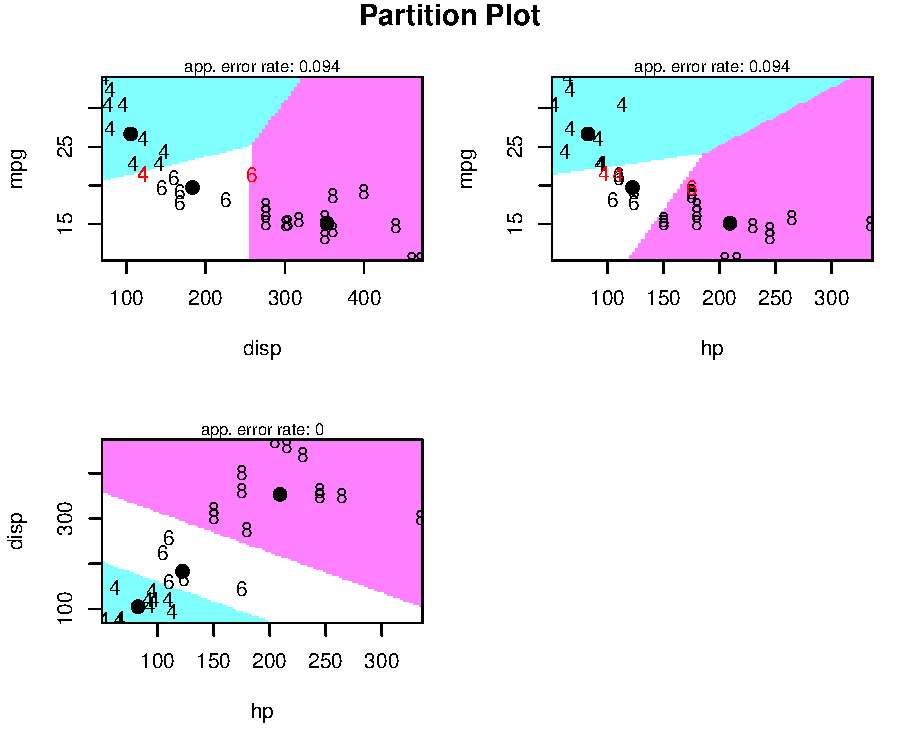
\includegraphics[width=\maxwidth]{figure/unnamed-chunk-71} 

}


\begin{kframe}\begin{alltt}
\hlkwd{partimat}\hlstd{(}\hlkwd{as.factor}\hlstd{(c}\hlopt{$}\hlstd{cyl)} \hlopt{~} \hlstd{.,} \hlkwc{data} \hlstd{= c,} \hlkwc{method} \hlstd{=} \hlstr{"qda"}\hlstd{,} \hlkwc{nplots.vert} \hlstd{=} \hlnum{2}\hlstd{)}
\end{alltt}
\end{kframe}

{\centering \includegraphics[width=\maxwidth]{figure/unnamed-chunk-72} 

}



\end{knitrout}


\end{document}
